%!TEX program = xelatex
% 完整编译: xelatex -> biber/bibtex -> xelatex -> xelatex
%\documentclass[lang=cn,a4paper,newtx]{elegantpaper}
\documentclass[letterpaper,12pt]{article}


% 添加中文支持
\usepackage[UTF8]{ctex} % 这是添加中文支持的关键

\usepackage{fullpage} % Package to use full page
\usepackage{parskip} % Package to tweak paragraph skipping
\usepackage{tikz} % Package for drawing
\usepackage{mathtools}
\usepackage{amsfonts}
\usepackage{fancyhdr}
\usepackage{times}
\usepackage{changepage}
\usepackage{amssymb}
\usepackage{amsthm}
%\usepackage[english]{babel}
\usepackage{graphicx}
\usepackage{xr-hyper}
\usepackage{hyperref}
%\theoremstyle{plain}

\newtheorem{theorem}{Theorem}
\newtheorem{lemma}{Lemma}
\newtheorem{assumption}{Assumption}

\def\mathbi#1{\textbf{\em #1}}

\newcommand{\bsa}{\boldsymbol{a}}
\newcommand{\bsb}{\boldsymbol{b}}
\newcommand{\bsc}{\boldsymbol{c}}
\newcommand{\bsd}{\boldsymbol{d}}
\newcommand{\bse}{\boldsymbol{e}}
\newcommand{\bsf}{\boldsymbol{f}}
\newcommand{\bsg}{\boldsymbol{g}}
\newcommand{\bsh}{\boldsymbol{h}}
\newcommand{\bsi}{\boldsymbol{i}}
\newcommand{\bsj}{\boldsymbol{j}}
\newcommand{\bsk}{\boldsymbol{k}}
\newcommand{\bsl}{\boldsymbol{l}}
\newcommand{\bsm}{\boldsymbol{m}}
\newcommand{\bsn}{\boldsymbol{n}}
\newcommand{\bso}{\boldsymbol{o}}
\newcommand{\bsp}{\boldsymbol{p}}
\newcommand{\bsq}{\boldsymbol{q}}
\newcommand{\bsr}{\boldsymbol{r}}
\newcommand{\bss}{\boldsymbol{s}}
\newcommand{\bst}{\boldsymbol{t}}
\newcommand{\bsu}{\boldsymbol{u}}
\newcommand{\bsv}{\boldsymbol{v}}
\newcommand{\bsw}{\boldsymbol{w}}
\newcommand{\bsx}{\boldsymbol{x}}
\newcommand{\bsy}{\boldsymbol{y}}
\newcommand{\bsz}{\boldsymbol{z}}

\newcommand{\bsA}{\boldsymbol{A}}
\newcommand{\bsB}{\boldsymbol{B}}
\newcommand{\bsC}{\boldsymbol{C}}
\newcommand{\bsD}{\boldsymbol{D}}
\newcommand{\bsE}{\boldsymbol{E}}
\newcommand{\bsF}{\boldsymbol{F}}
\newcommand{\bsG}{\boldsymbol{G}}
\newcommand{\bsH}{\boldsymbol{H}}
\newcommand{\bsI}{\boldsymbol{I}}
\newcommand{\bsJ}{\boldsymbol{J}}
\newcommand{\bsK}{\boldsymbol{K}}
\newcommand{\bsL}{\boldsymbol{L}}
\newcommand{\bsM}{\boldsymbol{M}}
\newcommand{\bsN}{\boldsymbol{N}}
\newcommand{\bsO}{\boldsymbol{O}}
\newcommand{\bsP}{\boldsymbol{P}}
\newcommand{\bsQ}{\boldsymbol{Q}}
\newcommand{\bsR}{\boldsymbol{R}}
\newcommand{\bsS}{\boldsymbol{S}}
\newcommand{\bsT}{\boldsymbol{T}}
\newcommand{\bsU}{\boldsymbol{U}}
\newcommand{\bsV}{\boldsymbol{V}}
\newcommand{\bsW}{\boldsymbol{W}}
\newcommand{\bsX}{\boldsymbol{X}}
\newcommand{\bsY}{\boldsymbol{Y}}
\newcommand{\bsZ}{\boldsymbol{Z}}



\newcommand{\bsigma}{\boldsymbol{\sigma}}
\newcommand{\bsPhi}{\boldsymbol{\Phi}}
\newcommand{\bsphi}{\boldsymbol{\phi}}
\newcommand{\bstau}{\boldsymbol{\tau}}

\newcommand{\sym}[1]{\operatorname{sym}#1}
\newcommand{\skw}[1]{\operatorname{skw}#1}
\newcommand{\diver}[1]{\operatorname{div}#1}
\newcommand{\grad}[1]{\operatorname{grad}#1}
\newcommand{\curl}[1]{\operatorname{curl}#1}
\newcommand{\tr}[1]{\operatorname{tr}#1}
\newcommand{\dev}[1]{\operatorname{dev}#1}
\newcommand{\sign}[1]{\operatorname{sign}#1}
%\newcommand{\span}[1]{\operatorname{span}#1}


\title{$H(\diver; \mathbb{S})$ 协调的对称张量有限元}
%\author{Chunyu Chen \\ Xiangtan University\ 数学与计算科学学院}

%\date{\today}

\begin{document}

\maketitle

%\begin{abstract}
%\end{abstract}

\section{引言}  
在线弹性方程的混合元方法中,应力 $\bsigma$ 和位移 $\bsu$ 的有限元空间分别为
$H(\diver; \mathbb{S})$ 和 $L^2$,其中 $\mathbb{S}$ 为对称张量空间。
对应的有限元空间 $\Sigma_h$ 和 $V_h$ 需要满足 
Infsup 条件,该条件成立的前提是 $\diver \Sigma_h = V_h$。

对于任意的单纯形 $T$,令 $\mathbb{B}_k(\diver, T) := \{ \sigma \in \mathbb{P}_k(T,
\mathbb{S})\mid \sigma|_{\partial T} \cdot \bsn = 0\}$
为迹零多项式空间,对于该空间有
$$
\diver \mathbb{B}_k(\diver, T) = \mathbb{P}_{k-1}(T, \mathbb{S}) \cap RM^{\perp}
$$
其中 $RM^{\perp}$ 为 $RM$ 的 $L^2$ 正交补空间,$RM:= \mathbb{P}_0(T, \mathbb{R}^d) + 
\mathbb{P}_0(T, \mathbb{K})\bsx$,$\mathbb{K}$ 为 $d$ 维反对称矩阵。
对于单纯形网格 $\mathcal{T}_h$,以及 $\mathcal{T}_h$ 上某个 $H(\mathrm{div},
\mathbb{S})$ 协调的有限元空间 $\Sigma_h$,作如下假设:
\begin{enumerate}
    \item[(A1)] \label{assumption1prim}$\diver \Sigma_T = \mathbb{P}_{k-1}(T, \mathbb{S}), \quad \forall T \in
        \mathcal{T}_h$.
    
    \item[(A2)] \label{assumption2}如下自由度在 $\Sigma_h$ 上是线性无关的: 
        $$
        \mathcal{N}_{F, \bsq}(\bsigma) := \int_{F} (\bsigma \cdot \bsn) \cdot \bsq
        \mathrm{d}S, \quad \forall \bsq \in \mathbb{P}_1 (T, \mathbb{R}^d), F \in
        \Delta_{n-1}\mathcal{T}_h。
        $$ 
\end{enumerate}
那么可以得到 $\diver \Sigma_h = \mathbb{P}_{k-1}^{-1}(\mathcal{T}_h, \mathbb{S})$。
其中假设 \hyperref[assumption2]{(A2)} 保证了 $\Pi_{T \in \mathcal{T}_h}
RM(T) \subseteq \diver \Sigma_h$。 

Hu-Zhang 元是一种 $H(\mathrm{div}, \mathbb{S})$ 协调有限元,其形函数空间为
$\mathbb{P}_k(T, \mathbb{S})$,因此自然满足假设 \hyperref[assumption1prim]{(A1)},当
$k \geq d+1$ 时,又满足假设 \hyperref[assumption2]{(A2)}。Hu-Zhang 元包含超光滑自由度,
其要求在网格的所有小于等于 $d-1$ 维的子单形上都法向连续,这些特点
均源自于形函数空间的对称性与光滑性。

%以二维,$k=2$ 为例,
%$P_2(T, \mathbb{S})|_{\partial T} \not= \Pi_{e \in \partial T} \mathbb{P}_2$ 是一个 $6$ 维的线性空间,而
%假设 \hyperref[assumption2]{(A2)} 中涉及的自由度有 $9$ 个,
%所以不能施加该点周围两条边的法向分量作为自由度 (4 个自由度),这是超光滑自由度的来源。
%
为了解决这个问题,形函数空间的选取可以在 $\mathbb{P}_k(T,
\mathbb{S})$ 的基础上,加上一些额外的 $H(\diver; \mathbb{S})$ 协调的函数。
这些函数非光滑,在 $\partial T$ 上的迹 $\bsigma \cdot \bsn$ 非零,
以使假设 \hyperref[assumption2]{(A2)} 中的自由度在 $k \leq d$ 时不再线性相关。且为了
\hyperref[assumption1]{(A1)}
成立,这些函数要求散度为零。下面给出这些函数的构造方法。

\section{可杂交化 $H(\diver; \mathbb{S})$ 协调有限元}
根据弹性复形的恰当性,$H(\diver; \mathbb{S})$ 协调且散度为零的函数组成
了空间 $U$ 在其对应的微分算子 $\mathrm{d}$ 下的
像,其中 $U$ 是弹性复形中 $H(\diver; \mathbb{S})$ 前面的空间。
\begin{equation}
    \label{eq:hilbertcomplex}
    U \xrightarrow{\mathrm{d}} H(\diver; \mathbb{S})
    \xrightarrow{\mathrm{div}} L^2(\mathbb{R}^d)
\end{equation}
因此,可以选取 $U$ 中的函数在 $\mathrm{d}$ 下的像作为额外的函数,
为了构造非无穷光滑函数引入如下的分裂单纯形。
\subsection{分裂单纯形}
对于一个 $d$ 维单纯形 $T$,其 $d+1$ 个顶点
为 $\bsx_0, \cdots, \bsx_d$,定义 
$$
\bsx_c = \frac{1}{d+1}\sum_{i=0}^d \bsx_i, \quad
\bst_{ij} = \bsx_j - \bsx_i, \quad \bst_{ic} =
\bsx_c - \bsx_i
$$
对于 $f \in \Delta(T)$,
定义 $\bst_{fc} = \bst_{f[0]c} = \bsx_c - \bsx_{f[0]}$。
通过连接 $\bsx_c$ 和 $\bsx_i$ 可以将 $T$ 分裂为 $d+1$ 个 $d$ 维单纯形,记为
$T^R$。
$T_i$ 为 $T^R$ 中不包含 $\bsx_i$ 的单纯形,对于 $f \in \Delta_{d-1} T$, $T_{f^*}$
包含 $f$。
$\chi_{T_i}$ 为 $T_i$ 上的特征函数。
\begin{figure}[h]
\centering
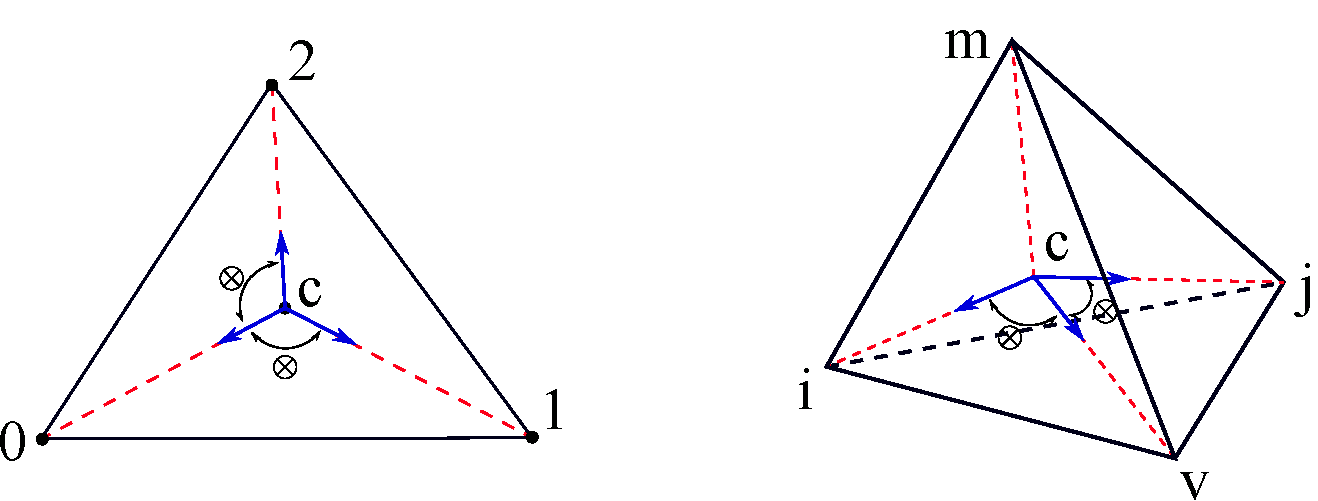
\includegraphics[width=0.7\textwidth]{./figures/splite_cell.pdf}
\caption{分裂单纯形}
\end{figure}

$\lambda_i$ 为 $T^R$ 上连续的分片线性函数,满足
$$
\lambda_i(\bsx_j) = \delta_{ij}, \quad \forall j = 0, \cdots, d, \quad 
\text{ and } \quad \lambda_i(\bsx_c) = 0.
$$
\begin{lemma}
\label{lem:dual}
对于 $T^R$ 中的一个四面体 $T_i, 0\leq i \leq d$,
$\{\bst_{cm}\}_{m=0, m\not=i}^d$ 是 $\mathbb{R}^d$ 中的一个基,且 
$\{\nabla \lambda_{m}|_{T_i}\}_{m=0, m\not=i}^d$ 是其对偶基。
\end{lemma}

\subsection{二维情况}
在二维情况下,弹性复形中 $U = H^2$,微分算子 $\mathrm{d} = J$ 定义如下: 
\begin{equation}
\label{eq:Jdef}
J(u) = 
\begin{pmatrix}
  0 & -1\\ 1 & 0
\end{pmatrix}
\nabla^2 u 
\begin{pmatrix}
  0 & 1\\ -1 & 0
\end{pmatrix}
\end{equation}

现在定义分裂三角形 $T^R$ 上的 $H^2$ 协调函数。
令三个顶点为 $\bsx_0, \bsx_1, \bsx_2$,
对于顶点 \textsf{v},令 $[i, j] = v^*$,定义
$$
\psi_{v} = \lambda_v^3 \lambda_i \chi_{T_j} - \lambda_v^3 \lambda_j \chi_{T_i}
$$
\begin{lemma}
    $\psi_v \in H^2(T^R)$.
\end{lemma}
\begin{proof}
    只需证明 $\nabla\psi_v$ 在 $T^R$ 上连续,即在边 $[v, c], [i, c], [j, c]$
    上跳量为零。
    $$
    \nabla \psi_v = 
    (3\lambda_v^2\lambda_i \nabla \lambda_v + \lambda_v^3 \nabla \lambda_i)
    \chi_{T_j} -
    (3\lambda_v^2\lambda_j \nabla \lambda_v + \lambda_v^3 \nabla \lambda_j)
    \chi_{T_i} 
    $$
    因为 $\lambda_v$ 在 $[i, c], [j, c]$ 上为零,所以 $\nabla\psi_v$
    在这两条边上跳量为零。在 $[v, c]$ 上 $\lambda_i$ 和 $\lambda_j$ 都是零,因此
    $[\![\nabla\psi_v]\!]|_{[v, c]} = \lambda_v^3 (\nabla \lambda_i + \nabla
    \lambda_j)$。因为 $T_i$ 和 $T_j$ 面积相同,所以 $\nabla \lambda_i$ 和 
    $\nabla \lambda_j$ 方向相反,大小相等,所以 $\nabla\psi_v$ 在 $[v, c]$ 上
    跳量为零。引理得证。
\end{proof}

显然 $\psi_v$ 与 $\mathbb{P}_k(T, \mathbb{S})$ 线性无关,更进一步的有以下引理:
\begin{lemma}
\label{lem:jump}
    不存在 $\bsq \in \mathbb{P}_k(T, \mathbb{S})$,
    使得 $(\bsq - J(\psi_v))|_{\partial T}\cdot \bsn = 0$。
\end{lemma}
\begin{proof}
$J(\psi_v)$ 在 $T^R$ 上不连续:
$$
J(\psi_v) : (\bst_{cv}\otimes \bst_{cv}) = 
\nabla^2 \phi_v : (\bsn_{cv}\otimes \bsn_{cv}) = \frac{\partial^2 \psi_v}{
\partial n_{cv}^2}
$$
因为 $\psi_v$ 在 $[v, c]$ 上二阶法向导数不连续,所以 
$J(\psi_v)|_{T_i}:
(\bst_{ci}\otimes \bst_{ci})$ 和 $J(\psi_v)|_{T_j}:
(\bst_{cj}\otimes \bst_{cj})$ 在 $\bsx_v$ 上不相等。
所以 $J(\psi_v)|_{\partial T}\cdot \bsn$ 在 $\partial T$ 上不连续。

若存在 $\bsq \in \mathbb{P}_k(T, \mathbb{S})$,使得 
$(\bsq - J(\psi_v))|_{\partial T}\cdot \bsn = 0$,
那么 $\bsq$ 在 $\partial T$ 上间断,显然不可能,因此引理得证。
\end{proof}

\begin{theorem}
\label{thm:hdivsdof2d}
    定义 $\Sigma_T = \mathbb{P}_k(T, \mathbb{S}) + 
    \mathrm{span}\{J(\psi_i)\}_{i=0}^2$,
    那么 $\Sigma_T \in H(\diver; \mathbb{S})$,且在 $\Sigma_T$ 上如下自由度是唯一可解的:
    \begin{align}
        (\bsigma\cdot \bsn, \bsq)  & \quad \forall e \in
        \Delta_1 T, \bsq \in \mathbb{P}_k(T, \mathbb{R}^2), \label{eq:dof1}\\
    (\bsigma : \bsq) & \quad \forall \bsq \in
    \mathbb{B}_k(\diver; T)\label{eq:dof2}
    \end{align}
\end{theorem}
\begin{proof}
    $H(\diver; \mathbb{S})$ 协调性显然,现在证明自由度的唯一可解性。
    首先统计自由度的个数,第一种自由度有 $6(k+1)$ 个,
    根据几何分解,
    第二种自由度有
    $\mathrm{dim}(\mathbb{B}_k(\diver; T)) = 3(k-1)(k-2)/2 + 3(k-1)$ 个,空间
    $\Sigma_T$ 的维数为 $3(k+1)(k+2)/2 + 3$,经过计算可知空间维数与自由度个数相同。
    令 $\bsigma \in \Sigma_T$ 且 $\bsigma$ 的自由度为零,因为 $\sigma \cdot \bsn\in
    \mathbb{P}_k(T, \mathbb{R}^2)$,所以自由度 \eqref{eq:dof1} 
    为零说明 $\bsigma \cdot \bsn
    |_{\partial T} = 0$,
    根据引理 \ref{lem:jump} 可知
    $\bsigma \in \mathbb{B}_k(\diver;
    T)$。而自由度 \eqref{eq:dof2} 为零说明 $\bsigma = 0$,因此自由度唯一可解性得证。
\end{proof}

定义 
$$
\Sigma_h := \{\bsigma \in L^2(\Omega) \mid \bsigma|_T \in \Sigma_T, \forall T \in
\mathcal{T}_h, \text{ and Dof} \eqref{eq:dof1} \text{ is single valued}\}.
$$
那么 $\Sigma_h$ 是一个 $H(\diver; \mathbb{S})$ 协调有限元空间。

\subsection{任意维的情况}
根据复形的方法可以将该方法推广到任意维的情况,但 $2$
维以上空间的弹性复形构造复杂,
本节给出另外一种构造性的方法。
首先考察前面章节中,在 $2$ 维情况下增加的函数 $J(\psi_v)$ 的形式,记 
$$
\nabla^{\perp}f = \begin{pmatrix}
-\frac{\partial f}{\partial y} \\ \frac{\partial f}{\partial x} \end{pmatrix} = 
    \begin{pmatrix}
        0 & -1\\ 1 & 0
    \end{pmatrix}\nabla f
$$
为 $\nabla f$ 的旋转。那么根据 $J$ 的定义 \eqref{eq:Jdef},有 
$$
\begin{aligned}
J(\psi_v) = & 6(\lambda_v^2 \sym(\nabla^{\perp} \lambda_i\otimes \nabla^{\perp}
    \lambda_v) + \lambda_v\lambda_i \nabla^{\perp} \lambda_v\otimes
\nabla^{\perp} \lambda_v)\chi_{T_j}\\
& - 6(\lambda_v^2 \sym(\nabla^{\perp}
\lambda_j\otimes \nabla^{\perp}
    \lambda_v) + \lambda_v\lambda_j \nabla^{\perp} \lambda_v\otimes
\nabla^{\perp} \lambda_v)\chi_{T_i}
\end{aligned}
$$
注意,存在常数 $c_1, c_2$,使得
$$
\nabla^{\perp} \lambda_v = c_1 \bst_{ci}\chi_{T_j} + c_2 \bst_{cj}\chi_{T_i}
$$
记:
$$
\begin{aligned}
    \psi_v^0 & = \lambda_v \lambda_i (\bst_{ci} \otimes \bst_{ci})\chi_{T_j},
    \quad 
    \psi_v^1 = \lambda_v \lambda_j (\bst_{cj} \otimes \bst_{cj})\chi_{T_i},\\
    \psi_v^2 & = \lambda_v^2 (\sym(\bst_{cv}\otimes \bst_{ci})\chi_{T_j} -
    \sym(\bst_{cv}\otimes \bst_{cj})\chi_{T_i})
\end{aligned}
$$
那么 $J(\psi_v)$ 是 $\psi_v^0, \psi_v^1, \psi_v^2$ 的一个线性组合,有一下引理:
\begin{lemma}
\label{lem:diver}
上面定义的函数 $\psi_v^0, \psi_v^1, \psi_v^2 \in H(\diver; \mathbb{S})$。
且存在某个线性组合散度为零。
\end{lemma}
\begin{proof}
只需证明在内部边 $[v, c], [i, c], [j, c]$ 上的法向连续。现在 $\psi_v^0$ 和
$\psi_v^1$ 在这三条边上都是零,而 $\psi_v^2$ 在 $[i, c]$ 和 $[j, c]$ 上
是零的,且在 $[v, c]$ 上,
$$
\begin{aligned}
    [\![\psi_v^2|_{[v, c]}\cdot \bsn_{[v, c]}]\!] & = \frac{1}{2}\lambda_v^2  
((\bst_{ci} + \bst_{cj}) \cdot \bsn_{[v, c]})\bst_{cv}
\end{aligned}
$$
因为 
$$
\bst_{ci} + \bst_{cj} = \bsx_c - \bsx_i + \bsx_c - \bsx_j = \bsx_v -
\bsx_c = -\bst_{cv}, 
$$
所以跳量为零。$H(\diver; \mathbb{S})$ 协调性得证。
因此可以计算三个函数的散度,根据 $\nabla \lambda_v|_{T_i} \perp \bst_{cj}$ 可得
$$
\begin{aligned}
    \diver(\psi_v^0) & = \lambda_v \bst_{ci} \chi_{T_j}, \quad 
    \diver(\psi_v^1) = \lambda_v \bst_{cj} \chi_{T_i},\quad
    \diver(\psi_v^2) & = \lambda_v (\bst_{ci} \chi_{T_j} - \bst_{cj} \chi_{T_i})
\end{aligned}
$$
显然 $\diver(\psi_v^2 - \psi_v^0 + \psi_v^1) = 0$。
\end{proof}

根据上面的引理可知,可以使用构造性的方法来构造我们需要的函数,其关键是张量部分
为 $\{\bst_{c0}, \bst_{c1}, \cdot, \bst_{cd}\}$ 之中的某两个向量的张量积,
因为这些向量与 $\{\nabla \lambda_0, \nabla \lambda_1, \cdots, \nabla
\lambda_d\}$ 具有某种对偶性见引理 \ref{lem:dual},使得构造的函数的散度易于计算。
现在我们将该构造方法推广到任意维。

考虑 $d$ 维单纯形 $T$,$e$ 是 $T$ 上的一个 $l$ 维面,$l < d-1$. 
对于 $\alpha \in \mathbb{T}_k^{l}$,定义
$$
\lambda^{\alpha}_e = \lambda_{e[0]}^{\alpha_0} \lambda_{e[1]}^{\alpha_1}
\cdots \lambda_{e[l]}^{\alpha_l}
$$
我们类似与上面的方法,定义三类 $H(\diver; \mathbb{S})$ 协调的函数:
对于 $\alpha \in \mathring{\mathbb{T}}_{k}^{l} = \{ \alpha \in \mathbb{T}_k^{l} \mid 
\alpha_i \not= 0, \forall i = 0, \cdots, l\}$,$i < j \in e^*$,
定义 
$$
\begin{aligned} 
    \psi_{ij, 0}^{e, \alpha} & = \lambda^{\alpha - \epsilon_0}_e\lambda_i
    \bst_{ci} \otimes \bst_{ci} \chi_{T_j}\\
    \psi_{ij, 1}^{e, \alpha} & = \lambda^{\alpha - \epsilon_0}_e\lambda_j
    \bst_{cj} \otimes \bst_{cj} \chi_{T_i}\\
    \psi_{ij, 2}^{e, \alpha} & = 
    \lambda_e^{\alpha}(\sym(\bst_{ce} \otimes \bst_{ci})\chi_{T_j} -
    \sym(\bst_{ce} \otimes \bst_{cj})\chi_{T_i})
\end{aligned}
$$
其中 $\epsilon_0 = (1, 0, \cdots, 0)$,是一个长度为 $l+1$ 的数组。
我们有以下引理:
\begin{lemma}
\label{lem:diver2}
$\forall \alpha \in \mathring{\mathbb{T}}_{k}^{l}$,$i < j \in e^*$,
上面定义的函数 $\psi_{ij, 0}^{e, \alpha}, \psi_{ij, 1}^{e, \alpha},
\psi_{ij, 2}^{e, \alpha} \in H(\diver; \mathbb{S})$。
且存在某个线性组合散度为零。
\end{lemma}
\begin{proof}
对于 $f \in \Delta T$ 定义 $\bar{f} = f\cup \{\bsx_c\} \in
\Delta \mathring{T^R}$ 为 $T^R$ 的一个内部面。
我们只需要证明
对于任意的 $f \in \Delta_{d-2} T$,三类函数在 $\bar{f}$ 上的法向连续。

首先讨论 $\psi_{ij, 0}^{e, \alpha}$ 的协调性,$\psi_{ij, 1}^{e, \alpha}$ 证明类似,
分情况讨论:
若 $\bar{f} \not\in \Delta_{d-1} T_j$ 那么显然 $\psi_{ij, 0}^{e, \alpha}$ 在
$\bar{f}$ 上为零。考虑 $\bar{f} \in \Delta_{d-1} T_j$ 的情况,
令 $q = T_i\setminus \bar{f}$,
若 $q = i$,那么 $\lambda_i$ 在 $\bar{f}$ 上为零,这说明 
$\psi_{ij, 0}^{e, \alpha}$ 在 $\bar{f}$ 上为零,
若 $q \not = i$,记 那么 $\nabla \lambda_q$ 
是 $\bar{f}$ 上的一个法向量,根据 引理 \ref{lem:dual} 中的对偶性,
$\nabla \lambda_q \cdot \bst_{ci} = 0$,所以 $\psi_{ij, 0}^{e, \alpha}$ 
在 $\bar{f}$ 上的法向分量为零。所以 $\psi_{ij, 0}^{e, \alpha} \in H(\diver;
\mathbb{S})$。

现在讨论 $\psi_{ij, 2}^{e, \alpha}$ 的协调性,分情况讨论:
若 $f \not \in i^*$ 且 $ f \not \in j^*$,那么根据定义 $\psi_{ij, 2}^{e, \alpha}$ 在
$\bar{f}$ 上为零。
考虑 $f \in j^*$ 的情况,即 $\bar{f} \in \Delta_{d-1} T_j$,记 $q = T_j\setminus
\bar{f}$,若 $q = e[0]$,那么 $\lambda_e^{\alpha}$ 在 $\bar{f}$ 上为零,从而
$\psi_{ij, 2}^{e, \alpha}$ 在 $\bar{f}$ 上为零。
若 $q \not = e[0]$ 且 $q \not = i$,由于 $\nabla \lambda_q$ 是 $\bar{f}$
上的一个法向量,根据 引理 \ref{lem:dual} 中的对偶性,
$\nabla \lambda_q \cdot \bst_{ce} = \nabla \lambda_q \cdot \bst_{ci} = 0$,
所以 $\psi_{ij, 2}^{e, \alpha}$ 在 $\bar{f}$ 上的法向分量为零。
若 $q = i$,那么 $f = [i, j]^*$。
对 $f \in i^*$ 的情况应用相同的论证方法,我们最终只需要对 $f = [i, j]^*$ 的情况
进行讨论。
此时 $\nabla \lambda_i|_{T_j}$ 和 $\nabla \lambda_j|_{T_i}$ 是 $\bar{f}$
上的法向量,且根据 $T_i$ 和 $T_j$ 体积相同可知 $\nabla \lambda_i|_{T_j} =
-\nabla \lambda_j|_{T_i}$,
由于 $ i, j \in e^*$,所以 
$$
\nabla \lambda_i|_{T_j} \cdot \bst_{ci} = \nabla \lambda_j|_{T_i} \cdot
\bst_{cj} = 0, \quad \nabla\lambda_i|_{T_j} \cdot \bst_{ci} = \nabla \lambda_j|_{T_i}
\cdot \bst_{cj} = 1
$$
取 $\bsn_{\bar{f}} = \nabla \lambda_i|_{T_j}$,那么:
$$
\begin{aligned}
    [\![\psi_{ij, 2}^{e, \alpha}\cdot \bsn_{\bar{f}}]\!]|_{\bar{f}} & = \frac{1}{2}\lambda_e^{\alpha}
    ((\bst_{ci} + \bst_{cj}) \cdot \bsn_{\bar{f}})\bst_{ce}
    & = \frac{1}{2}\lambda_e^{\alpha} (\bst_{ci} + \bst_{cj}) \cdot
    \nabla\lambda_i|_{T_j} \bst_{ce}
    & = 0
\end{aligned}
$$
协调性得证。
现在计算三类函数的散度,
根据引理 \ref{lem:dual} 中的对偶性,由于 $i, j \in e^*$ 所以 
$$
\begin{aligned}
    \diver(\psi_{ij, 0}^{e, \alpha}) & = \lambda_e^{\alpha - \epsilon_0} \bst_{ci} \chi_{T_j},\\
    \diver(\psi_{ij, 1}^{e, \alpha}) & = \lambda_e^{\alpha - \epsilon_0} \bst_{cj} \chi_{T_i},\\
    \diver(\psi_{ij, 2}^{e, \alpha}) & = \frac{\alpha_0}{2} \lambda_e^{\alpha -
    \epsilon_0} (\bst_{ci} \chi_{T_j} - \bst_{cj} \chi_{T_i}) 
\end{aligned}
$$
令
$
\psi_{ij}^{e, \alpha} = -\frac{\alpha_0}{2}\psi_{ij, 0}^{e, \alpha} +
\frac{\alpha_0}{2}\psi_{ij, 1}^{e, \alpha} + \psi_{ij, 2}^{e, \alpha}
$
那么 $\diver(\psi_{ij}^{e, \alpha}) = 0$。
\end{proof}

\begin{lemma}
    \label{lem:jump}
    不存在 $\bsq \in \mathbb{P}_k(T, \mathbb{S})$,
    使得 $(\bsq - \psi_{ij}^{e, \alpha})|_{\partial T}\cdot \bsn = 0$。
\end{lemma}
\begin{proof}
    证明与引理 \ref{lem:jump} 类似。
\end{proof}

\begin{theorem}
\label{thm:hdivsdofnd}
    令 $V_T := \mathbb{P}_k(T, \mathbb{S}) + \oplus_{l = 0}^{d-2} \oplus_{e \in
    \Delta_{l} T} \mathrm{span}(\Phi_e^k)$,其中:
    $$
    \Phi_e^k = \{\psi_{ij}^{e, \alpha} \mid i < j \in e^*, \alpha \in
    \mathring{\mathbb{T}}_k^{l}\}
    $$
    那么 $V_T \in H(\diver; \mathbb{S})$。
    且在 $V_T$ 上如下自由度是唯一可解的:
    \begin{align}
        (\bsigma\cdot \bsn, \bsq)_F  & \quad \forall F \in
        \Delta_{d-1} T, \bsq \in \mathbb{P}_k(T, \mathbb{R}^d), \label{eq:dof3}\\
    (\bsigma : \bsq) & \quad \forall \bsq \in
    \mathbb{B}_k(\diver; T)\label{eq:dof4}
    \end{align}
\end{theorem}
\begin{proof}
    证明与 定理 \ref{thm:hdivsdof2d} 类似。
\end{proof}

定义全局空间
$$
\Sigma_h := \{\bsigma \in L^2(\Omega) \mid \bsigma|_T \in V_T, \forall T \in
\mathcal{T}_h, \text{ and Dof} \eqref{eq:dof3} \text{ is single valued}\}
$$


\begin{theorem}
    \label{thm:infsup}
    $\diver \Sigma_h = \mathbb{P}_{k-1}^{-1}(\mathcal{T}_h, \mathbb{S})$,且
    存在常数 $C > 0$,使得
    \begin{equation}
        \label{eq:infsup}
        \sup_{\bstau \in \Sigma_h} 
        \frac{(\diver \bstau, \bsv)}{\|\bstau\|_{H(\diver{})}}
        \geq C \|\bsv\|_{L^2}
    \end{equation}
\end{theorem}
\begin{proof}
\end{proof}








\section{数值实验}
\subsection{线弹性方程的混合元方法}
设 $\Omega$ 为 $\mathbb{R}^d$($d=2,3$)中的多边形区域,边界为 $\partial \Omega$,我们考虑以下弹性问题:  
$$
\left\{
\begin{aligned}
  \mathcal{A}(\bsigma) - \varepsilon(\bsu) & = 0, \quad \text{in} \quad \Omega, \\
  -\mathrm{div}\bsigma &= \bsf, \quad \text{in} \quad \Omega, \\
  \bsu &= 0, \quad \text{in} \quad \partial \Omega,
\end{aligned}
\right.
$$  
其中,$\bsigma$ 是应力张量,$u$ 是物体的位移向量,$f$ 是体力,$\varepsilon(u)$ 和 
$\mathcal{A}(\bsigma)$ 定义如下:
$$
\varepsilon(\bsu) = \frac{1}{2}(\nabla \bsu + \nabla \bsu^T),\quad
\mathcal{A}(\bsigma) = \lambda_0 \bsigma - \lambda_1\mathrm{tr}(\bsigma) I.
$$
令 $\lambda$ 和 $\mu$ 是拉梅(Lamé)常数,
上式中 $\lambda_0 = \frac{1}{2\mu}$ 和 $\lambda_1 = \frac{\lambda}{2\mu(2\mu +
d\lambda)}$,
$I$ 是单位张量。  
将 $\Omega$ 划分为一组单纯形网格 $\mathcal{T}_h$,并定义空间 $\Sigma_h$ 和
$V_h := \mathbb{P}_{k-1}^{-1}(\mathcal{T}_h)$,
线弹性方程的混合元方法为:找到 $\bsigma_h \in \Sigma_h$ 和 $\bsu_h \in V_h$,使得
\begin{equation}
\begin{aligned}
    a(\bsigma_h, \bstau_h) + b(\bstau_h, \bsu_h) &= 0, \quad \forall \bstau_h
    \in \Sigma_h,\\
    b(\bsigma_h, \bsv_h) &= (-\bsf, \bsv_h), \quad \forall v \in V_h,
\end{aligned}
\end{equation}
其中
$$
a(\bsigma_h, \bstau_h) = (\mathcal{A}(\bsigma_h), \bstau_h), \quad
b(\bstau_h, \bsu_h) = (\mathrm{div} \bstau_h, \bsu_h) 
$$
\subsection{二维}
令真解为 $u = (\sin(5x)\sin(7y), \cos(5x)\cos(4y))$,
$\Omega = (0, 1)^2$,
$\lambda_0 = 4$,$\lambda_1 = 1$。
图 \ref{fig:k235} 给出了 $k=2, 3, 5$ 时的数值结果,中可以看到,
$||\bsigma - \bsigma_h||_{L^2} = O(h^{k+1})$ 和 $||\bsu - \bsu_h||_{L^2} =
O(h^k)$。

\begin{figure}[h]
\centering
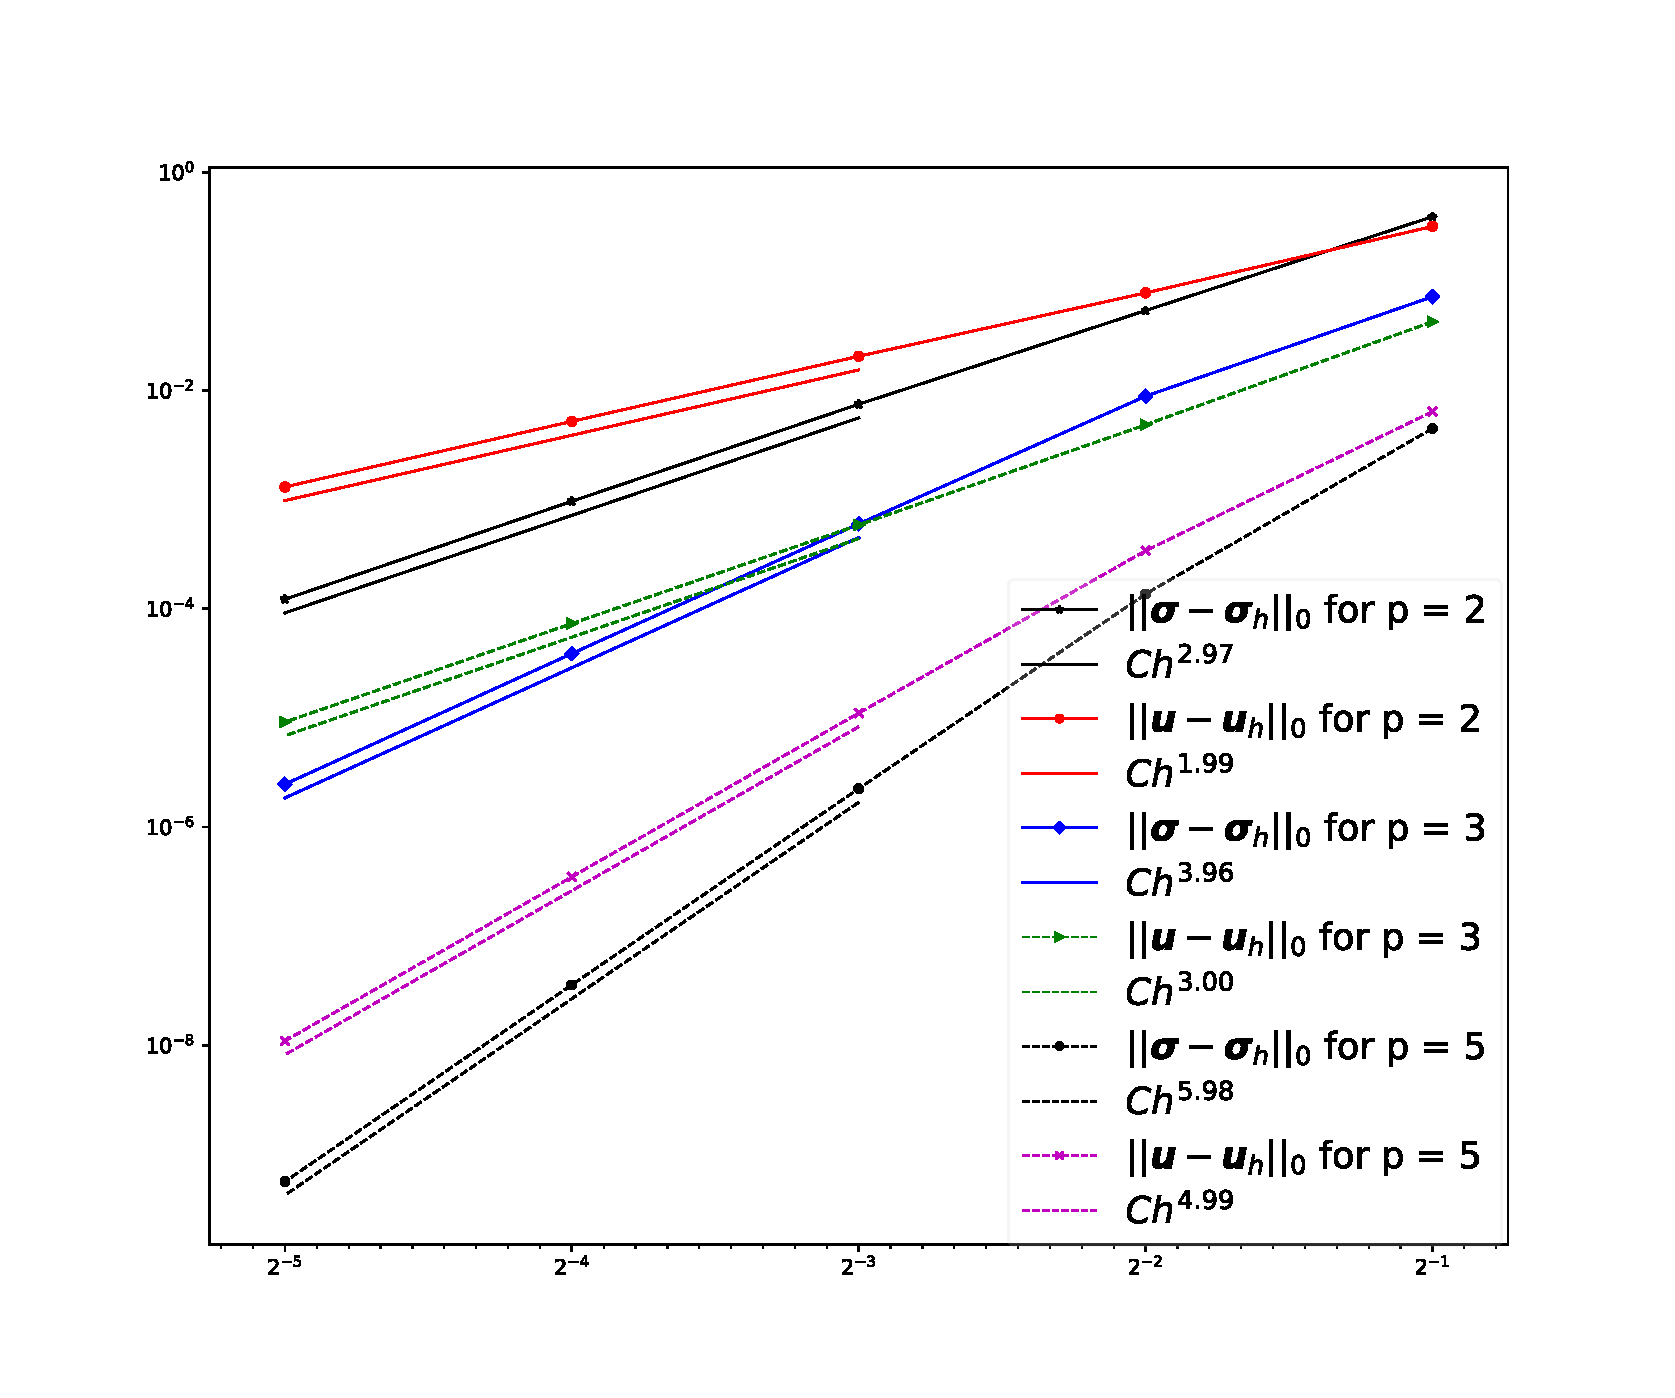
\includegraphics[width=0.7\textwidth]{./figures/divs.pdf}
\caption{$k=2, 3, 5$ 时的数值结果}
\label{fig:k235}
\end{figure}
























\end{document}
